%!TEX root = ../report.tex

\section{Link Layer}
Terminology:
\begin{itemize}
  \item Hosts and routers are nodes
  \item Communication channels between adjacent nodes are links
  \item A layer 2 packet is a frame and encapsulates a layer 3 packet called datagram
\end{itemize}

The data-link layer has the responsibility of transferring a datagram from one node to an adjacent node over a link.

\subsubsection*{Services}
\begin{itemize}
  \item Framing, link access, MAC addressing
  \item Reliable delivery between adjacent nodes (mostly in wireless transmission)
  \item Flow control: Pacing between sending and receiving nodes
  \item Error detection
  \item Error correction
  \item Half- and full-duplex (half = both ends can transmit, but not simultaneously)
\end{itemize}

\subsubsection*{Multiple Access Protocols}
When sharing a single channel, a distributed algorithm manages how nodes share it.
This management is done via the same channel as the actual communication and does not require a separate one coordination.

\subsubsection*{Medium Access Control (MAC) Protocols Taxonomy}
\begin{description}
  \item[Channel Partitioning] divides channel into smaller pieces (time, frequency, \dots)
  \item[Random Access] does not divide channels, but try to recover from collisions
  \item[Taking turns] Nodes take turns, requesting turns by polling or token passing
\end{description}

\subsection{Ethernet}
\begin{figure}[H]
  \centering
  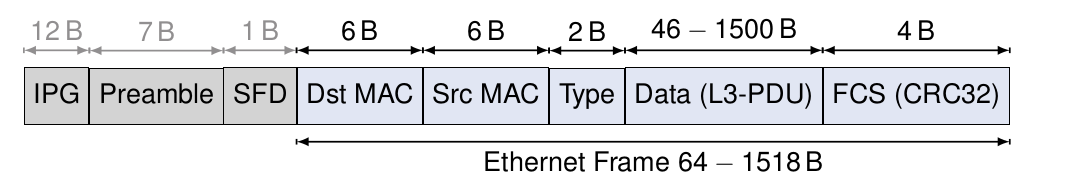
\includegraphics[width=.8\textwidth]{figures/ethernet_frame.png}
  \caption{Ethernet Frame}\label{fig:ethernet_frame}
\end{figure}
IPG = Inter packet gap, minimum idle period
Preamble = 7 byte (10101010\dots)
SFD = Start-of-frame delimiter (10101011)
Type = Ethernet II:\@ Protocol type of payload, Ethernet I:\@ length of payload in bytes
PAD = Padding if data length smaller than 46 byte
FCS = Frame check sequence (CRC-32)

There are several Ethernet standards, but they all share a common MAC protocol and frame format.
They provide different bandwidth (from 10M to 200/400G (planned for 2017)) and have different physical layer media like twisted pairs (xBase-T), optical fibres or even chip to chip interfaces on NIC.

\subsubsection{Carrier Sense Multiple Access - Collision Detection (CSMA/CD)}
CSMA/CD is used for detecting and reacting to collisions.
Its steps are
\begin{enumerate}
  \item NIC receives datagram and creates frame
  \item If NIC sees channel idle, it starts transmission, if channel busy, wait until idle
  \item If NIC does not detect another transmission during its own transmission, it is done
  \item If NIC does detect another transmission, jam signal is sent and transmission is aborted
  \item NIC enters exponential backoff: after m-th collision, NIC chooses k at random from 0, 1, \dots $2^m - 1$ and waits $k \cdot 512bit$ times and returns to step 2.
    Bit time is 0.1$\mu s$ for 10MbE
\end{enumerate}

\subsection{Limitations of Layer 2}
\begin{itemize}
  \item Flat addresses
  \item No hop count (dangerous when having loops)
  \item Missing protocols like ICMP
  \item Missing features: fragmentation, error messages, congestion feedback
\end{itemize}

\subsection{MAC addresses}
MAC addresses are 6 Byte long unique identifiers for NICs.
Manufacturers can buy portions of the total MAC address space from the IEEE Registration Authority, which assures uniqueness.
The first 3 bytes of the address in transmission order represent the Organization Unique Identifier (OUI).
If the 2nd least significant byte is 0, the MAC is OUI enforced, otherwise its locally administered.
MACs are transmitted in canonical form which stands for sending the least significant bit of each byte first (in memory, token ring and FDDI it is the other way around).

\subsection{Layer 2 Switching}
\subsubsection*{Hubs}
Hubs are repeaters which means they send every bit arriving out to all other links.
Because of this, frames from all connected nodes can collide with each other.
Furthermore there is no frame buffering or CSMA/CD.

\subsubsection*{Switch}
Switches are a lot smarter when compared to routers.
They store and forward Ethernet frames only to the node that the destination MAC address belongs to.
Furthermore they use CSMA/CD to access links.
Hosts do not need to be aware of the presence of switches and they do not need to be configures and learn themselves.
Learning is done when receiving packets: The switch then knows the location of the sender MAC address and stores it in a switch table.
An entry expires after a specified amount of time.
If a packet arrives, the switch table is checked if the destination is known.
If yes, the packet is only sent to that node, otherwise it is sent to all.

\vspace{10pt}
If more switches are involved, the \textbf{spanning tree protocol} is used.
It calculates a loop-free subnet of the given physical network and determines routing.
The calculation steps are as followed:
\begin{enumerate}
  \item Select root bridge, i.e.\ bridge with lowest bridge\_ID (concatenation of 16bit bridge\_priority and MAC address)
  \item determine least cost paths to root
  \begin{itemize}
    \item Every bridge determines cost of each path to root
    \item Every bridge picks least cost path
    \item port connecting to that path is root port 
    \item Bridges on network segment determine bridge port with least-cost-path to root, i.e.\ designated port
  \end{itemize}
  \item disable all other ports
\end{enumerate}

Bridge Protocol Data Units (BPDUs) are used to transmit configuration information about bridge\_IDs and root path costs, to notify about topology changes (TCN = Topology Change Notification) and for TCN acknowledgements.
